\documentclass[mscthesis, 11pt]{usiinfthesis}
\usepackage{lipsum}


\usepackage{listings}

\lstdefinelanguage{algebra}
{morekeywords={import,sort,constructors,observers,transformers,axioms,if,
else,end},
sensitive=false,
morecomment=[l]{//s},
}



\title{My Dissertation - A very long title\\ which runs over two
  lines} %compulsory
\specialization{Dependable Distributed Systems}%optional
\subtitle{Subtitle: Reinventing the World} %optional 
\author{Master Student} %compulsory
\begin{committee}
\advisor{Prof.}{Student's}{Advisor} %compulsory
\coadvisor{Prof.}{Student's}{Co-Advisor}{} %optional
\end{committee}
\Day{Yesterday} %compulsory
\Month{September} %compulsory
\Year{2010} %compulsory, put only the year
\place{Lugano} %compulsory

\dedication{To my beloved} %optional
\openepigraph{Someone said \dots}{Someone} %optional

%\makeindex %optional, also comment out \theindex at the end

\begin{document}

\maketitle %generates the titlepage, this is FIXED

\frontmatter %generates the frontmatter, this is FIXED

\begin{abstract}
This is a very abstract abstract. 
\end{abstract}


\begin{acknowledgements}
	Hi Mom!
\end{acknowledgements}

\tableofcontents 
\listoffigures %optional
\listoftables %optional

\mainmatter

\chapter{Introduction}
\section{Motivation}
PltRedex is domain-specific language embedded into Racket designed for specifying and debugging operational semantics. By specifying a language and reduction rules, PltRedex is able to apply reduction rules to terms by rewriting them. (FIXME) PltRedex also provides randomized testing functionality.

However, after testing PltRedex specification one might want to turn it into stand-alone interpreter and that's when dependency on Racket turns into a problem for the following reasons:

\begin{enumerate}
\item 
One have to ship entire Racket runtime to be able to run the specification.
\item
Racket is not particularly fast. 
\end{enumerate}

PyPltRedex is the tool that attempts to solve the problem by taking PltRedex specification and compiling it into RPython language - statically analyzable subset of Python programming language that is used for implementation of interpreters within the PyPy toolchain. Using RPython toolchain, resulting RPython program is then compiled into stand-alone, more efficient and considerably more low-level version of the program. However, by removing Racket from the equation, the specification has to be modified to use RPython instead.

\section{Goals}
Since PltRedex has existed for a while and provides wide range of functionality ranging from language specification, type checking and testing, PyPltRedex implements tiny subset of PltRedex that is enough to be usable. In particular,

\begin{itemize}
\item Only a subset of pattern language provided by PltRedex is supported.
\item
Only functionality required for term rewriting is supported.
\end{itemize}

\section{Thesis Outline}
TODO

\chapter{Features of PltRedex}

\section{Imp}

To introduce PLTRedex, Imp language will be used, originally introduced by Glynn Winskel.

\begin{lstlisting}
a = X | n | a1 + a2 | a1 * a2
b = true | false | a1 <= a2 | not b | b1 and b2 | b1 or b2
c = skip | x = a | c1; c2 | if b c1 else c2 | while b c


a in Aexp arithmetic expressions
b in Bexp boolean expressions
c in Com  commands 
X in Loc  locations
n in Z
\end{lstlisting}

\[\begin{prooftree}\infer0{ \vdash A }\hypo{ \vdash B } \infer1{ \vdash B, C }\infer2{ \vdash A\wedge B, C }\end{prooftree}\quad \rightsquigarrow \quad\begin{prooftree}\infer0{ \vdash A } \hypo{ \vdash B }\infer2{ \vdash A\wedge B }\infer1{ \vdash A\wedge B, C }\end{prooftree} 
\]

\[ 
\begin{prooftree}
\hypo{ \vdash B } \infer1{ \vdash B, C }
\end{prooftree}
\]

Set of states $\Sigma$ consists of of functions $\sigma$: \texttt{Loc -> Z}. Thus, $\sigma(X)$ is contents of location $X$ in state $\sigma$. 

Given arithmetic expression $a$ and state $\sigma$, define evaluation relation $<a,\sigma> \rightarrow n$: arithmetic expression $a$ in state $\sigma$ evaluates to integer $n$.

Similarly, define evaluation relation for boolean expressions $b$. $<b, \sigma> \rightarrow {true, flase}$: boolean expression $b$ in state $\sigma$ evaluates to either \texttt{true} or \texttt{false}.

Finally, define evaluation relation for command $c$. Given $c$ and state $\sigma$, $<c, \sigma> -> \sigma\prime$. 

Small-step operational semantics are specified below using inference rules.

TODO-this is quite lengthy. Also provide derivation tree for some example - say \texttt{x = 12; if x <= 20 x = x + 1 else x = x - 1 } showing resulting state after evaluation.


\section{Evaluation Contexts}

Inference rules above are verbose and can be tricky to evaluate. PLTRedex uses \texttt{evaluation contexts}, originally introduced in \texttt{https://www2.ccs.neu.edu/racket/pubs/tcs92-fh.pdf}. 

An evaluation context $E[.]$ is an expression containing a single occurence of special symbol $.$ called "hole".$E[e]$ is the expression that results from replacing $.$ with some expression $e$. Evaluation contexts are usually specified using EBNF grammar. 

Using evaluation contexts, the following inference is introduced

$(r, \sigma) \rightarrow (t\prime, \sigma) THEN (E[r], \sigma\prime) \rightarrow (E[t\prime], \sigma\prime)$. Where redex $r$ reduces to some expression $r$ in a single step.

This allows for specification one one global reduction rule seen above and reduction rule for each redex $r$. These are shown in Figure TODO.

\begin{lstlisting}

(x, sigma) -> (n, sigma) where n = sigma(x)
(n1 + n2, sigma) -> (n, sigma) where n = n1 + n2, n1, n2, n in Z.
(b1 and b2, sigma) -> (b, sigma) where b = b1 and b2.
(skip;c, sigma) -> (c, sigma)

E = []
  | (x = E)
  | E;c
  | (E + e)
  | (n + E)
  | (E * e)
  | (n + E)
  | if E c else c
 
TODO complete this.
\end{lstlisting}


\subsection{Imp: PLTRedex Implementation}

Basically include \texttt{https://github.com/mamysa/PyPltRedex/blob/master/examples/imp/imp-racketcompat.rkt} here but explain all the forms.

Also mention non-determinism.


\chapter{PyPy and RPython}
PyPy consists of two parts. 

PyPy Python Interpreter is an alterative to standard CPython implementation that aims to closely emulate behavior of CPython, written in RPython. It consists of three components: (1) bytecode compiler compiling source code of user application into Python code objects; (2) Python code objects interpreter; (3) standard object space that creates or manipulates Python objects.

RPython is a subset of Python that can be analyzed statically. The goal of RPython toolchain is to translate RPython programs into more efficient programs for various target platforms, generally ones that are considerably lower-level than Python. Compilation is carried out in the following stages:

\begin{enumerate}
\item Annotation pass performs a global analysis starting from a specified entry point inferring type of each variable and building a control flow graph. Control flow graph consists of \textit{basic blocks} that do not contain Python bytecode but rather operations after performing \textit{abstract interpretation} of the Python bytecode. Basic block always ends with jumps to other basic blocks. After construction of the flow graph has been completed, each encountered variable is annotated with the types of all possible Python objects that can be assigned to it.

\item 
The RPython Typer (or RTyper) uses the high-level information inferred during annotation phase to turn the operations in the control flow graphs into low-level operations. At this point, function inlining, \texttt{malloc} removal and other optimizations are applied. 

\item
Finally, the C backend takes flow graphs produced by \texttt{RTyper} and produces a number of C source files that are compiled into executable.
\end{enumerate}

Throughout the thesis RPython is treated as a black box. 

\section{Compile-Time Representation of RPython}

PyPltRedex works with \textbf{abstract syntax trees} and then emits RPython source code by traversing the tree and emitting strings. Abstract syntax tree itself is a tree that represent constructs of the language such as arithmetic operations, assignments, loops, etc.

In Python and other imperative languages, nodes of an abstract syntax tree can be split into two categories:

\begin{enumerate}
\item
Statements such as \texttt{while} and \texttt{for} loops, \texttt{if} statements, variable assignments.
\item
Expressions such as arithmetic operations, array element access, literal values such as integers or strings, etc.
\end{enumerate}

This allows for deeply nested expressions and can be quite tedious to work with. PyPltRedex's AST definition is modified to include \texttt{PyValue} - subset of expressions that includes only variables and literals. Expressions such as additions are thus now required to use \texttt{PyValue}, thus making resulting RPython code similar to typical three-address code intermediate representation that most compilers employ. Figure \ref{class-diagram-rpython} shows class diagram of all RPython abstract syntax tree nodes.

\begin{figure}[ht]
	\centering
	\makebox[\textwidth][c] { 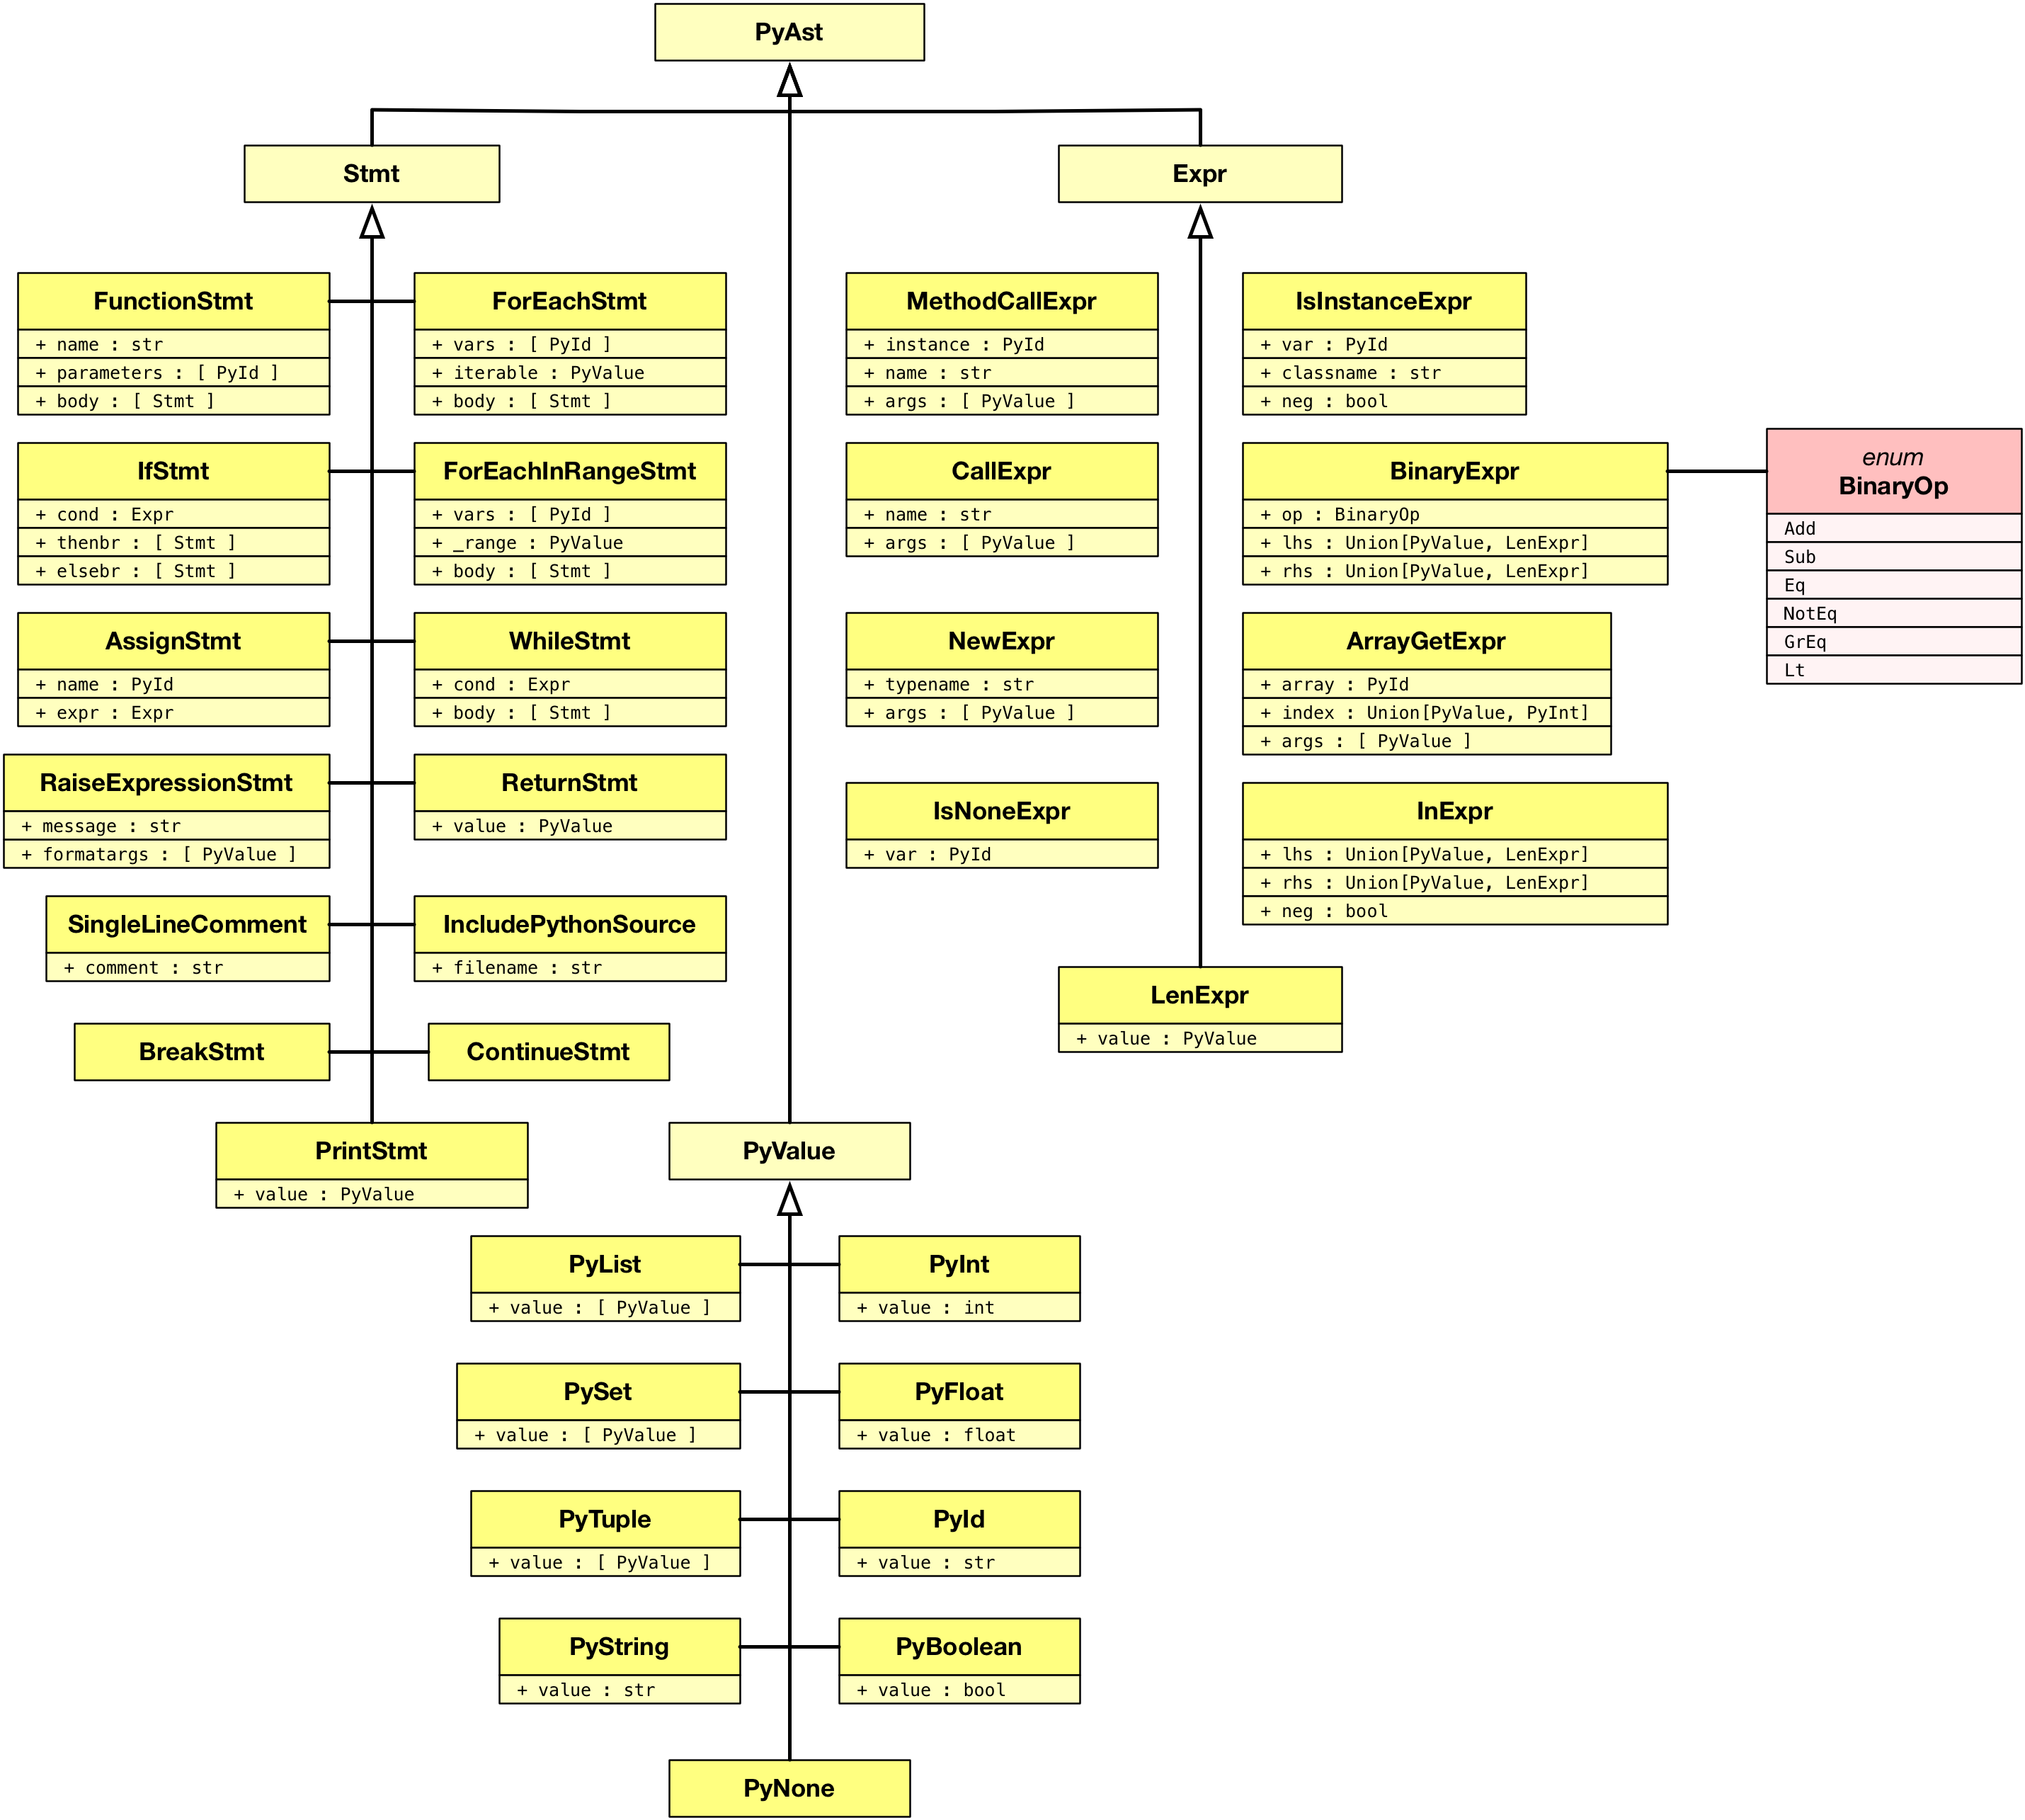
\includegraphics[scale=0.16]{class-diagram-rpython.png} }
	\caption{RPython abstract syntax tree.}
\label{class-diagram-rpython}
\end{figure}


\chapter{PyPltRedex Runtime}

This chapter goes over runtime. TODO

\section{Runtime Representation of Terms}
\label{section:runtime-terms}

All runtime terms are represented as shown in the class diagram in Figure \ref{class-diagram-runtime-term}

\begin{figure}[H]
	\centering
	\makebox[\textwidth][c] { 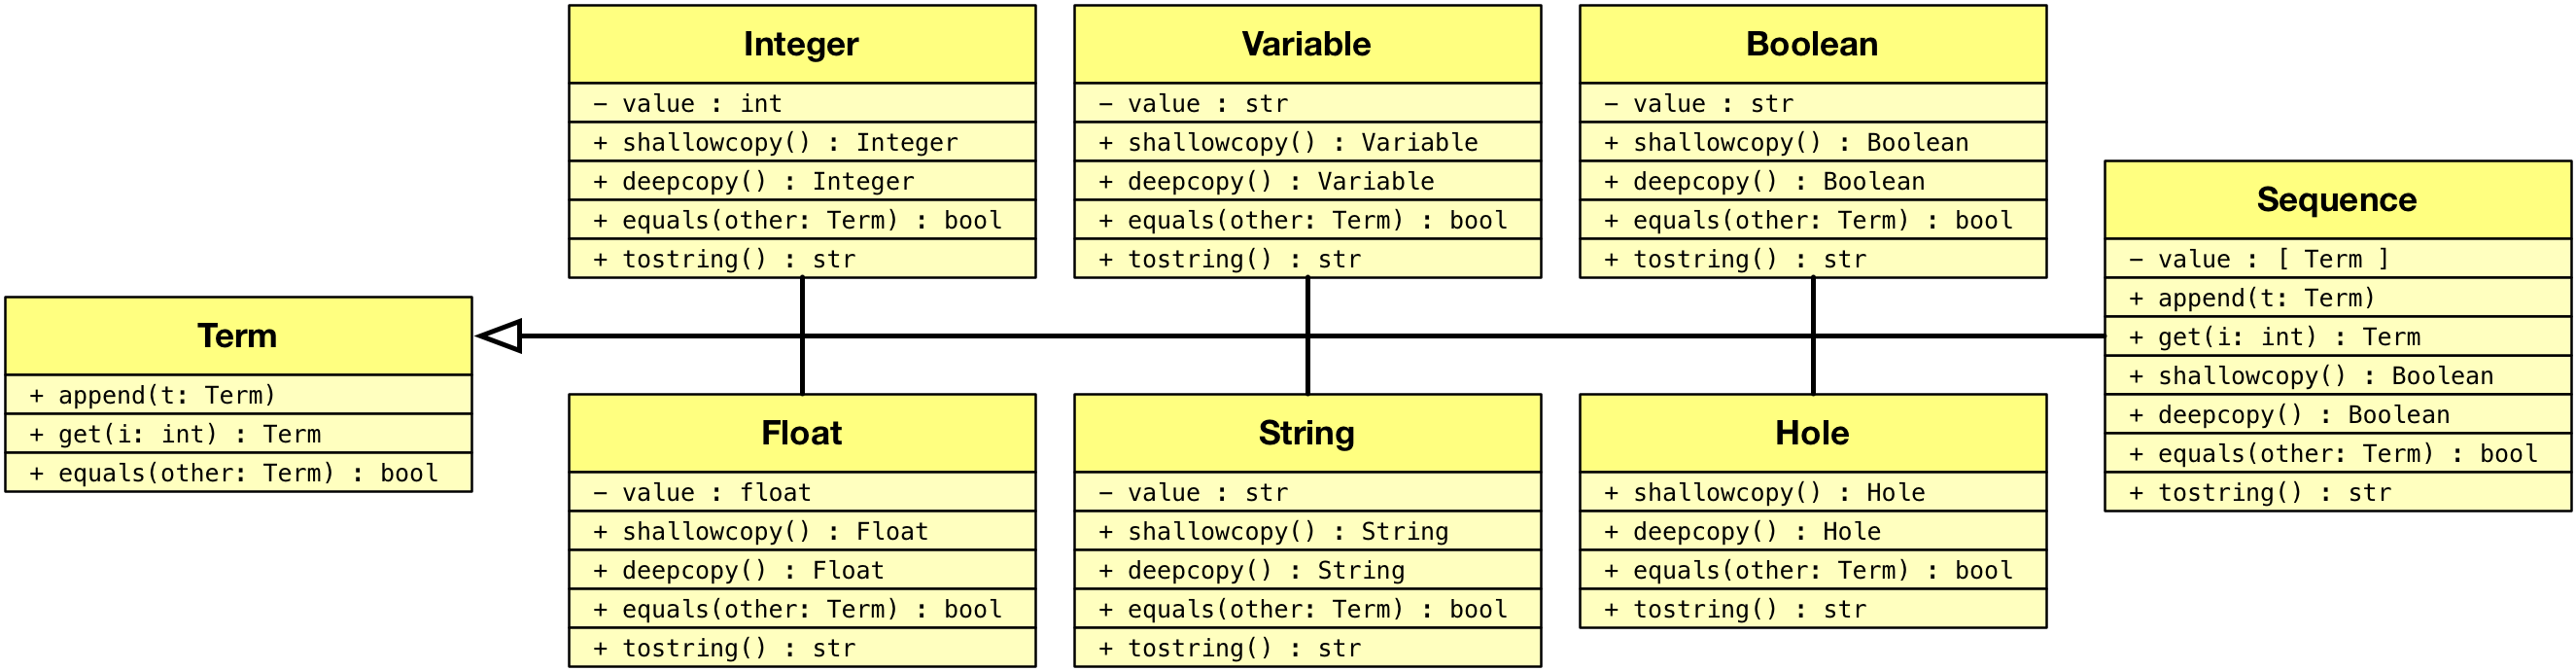
\includegraphics[scale=0.17]{class-diagram-runtime-term.png} }
\caption{\texttt{Term} class hierarchy.}
\label{class-diagram-runtime-term}
\end{figure}

These classes are all very similar and essentially just act as a wrapper for some primitive type. \texttt{Term} is the base class. Due to how RPython's type inference works creating a single class to represent all child classes such as \texttt{String} or \texttt{Float} results in the following compilation error.  Since the \texttt{LeafNode} instance is created with \texttt{helloworld!} string, any other instantiation of \texttt{LeafNode} expects it's second argument to be of type \texttt{string}. 

One may notice that, for example, \texttt{String} and \texttt{Variable} could be merged into one class and an additional \texttt{tag} field could be introduced to differentiate between strings and variables. However, since \texttt{isinstance} function is supported by RPython, such change would make term comparison logic more complex.

\begin{minted}[tabsize=2,obeytabs,fontsize=\normalsize]{python}
class LeafNode:
    def __init__(self, kind, value):
        self.kind = kind 
        self.value = value

def entrypoint():
    p = LeafNode('hello world!')
    q = LeafNode(12.5)

# UnionError:
#  SomeString(const='hello world!', no_nul=True)
#  SomeFloat(const=12.5)
\end{minted}

All classes implement following methods.
\begin{itemize}
\item \texttt{shallow\_copy} returns an exact copy of the term. This kind of copying is not recursive.
\item
\texttt{deep\_copy} copies the term recursively. In practice, it duplicates \texttt{shallow\_copy} for every term type except \texttt{Sequence}; each term in the sequence is deep-copied and new \texttt{Sequence} instance is returned containing copied terms.
\item
\texttt{equals} compares two terms based on the type of the term and then on the value.
\item
\texttt{tostring} returns a string representing the term. These are made to look like actual Racket expressions.
\end{itemize}
 
In addition, the following utility functions are provided to make implementation of certain functionalities easier.

\begin{itemize}
\item
	\texttt{copy\_path\_and\_replace\_last}. Given a path of terms $t_1, ..., t_n$  where terms $t_1, ..., t_{n-1}$ are expected to be of type \texttt{Sequence}, and given term $t_n^{\prime}$, the path is copied using \texttt{shallow\_copy} up to $t_n$, producing terms $t_1^\prime, ..., t_{n-1}^\prime$ and $t_n$ is replaced with $t_n^{\prime}$. All pointers to successor terms are also fixed up; that is, given two copied terms $t_i^{\prime}$ and $t_{i+1}^{\prime}$, $t_i^{\prime}$ will point to $t_{i+1}^{\prime}$ instead of $t_{i+1}$. $t_1^\prime$ is returned.
\item
	\texttt{locatehole} recursively traverses the term $t$ looking for term of type \texttt{Hole}. Each term on the path to \texttt{Hole} is recorded and upon successful search the path is returned.
\item
	\texttt{plughole}. Given two terms $t_1$ and $t_2$, first \texttt{locatehole} is called with $t_1$ as argument. If resulting path is non-empty, the result of \texttt{copy\_path\_and\_replace\_last} called with resulting path and $t_2$ is returned. Otherwise, $t_1$ is returned.
\item
	\texttt{asserttermsequal}. Given two terms, \texttt{equals} method is called and an Exception is raised if \texttt{equals} returns False.
\item
	\texttt{asserttermlistsequal}. Given two lists $T_1$, $T_2$ containing \texttt{Term} instances, \\ \texttt{asserttermsequal} function is called for each pair $t_1 \in T_1$ and $t_2 \in T_2$. Both lists are expected to have same lengths.
\item 
	\texttt{asserttermsequalpairwise}. Given a list $T$ containing \texttt{Term} instances, asserts that each pair $t_i, t_{i+1} \in T$ is equal, using \texttt{equals} method described previously.
\end{itemize}

\section{Runtime Representation of Matches}
\label{section:Match}

To implement matches, two classes are defined - \texttt{Match} and \texttt{Binding}, as seen in Figure \ref{class-diagram-match-binding}.

\begin{figure}[H]
	\centering
	\makebox[\textwidth][c] { 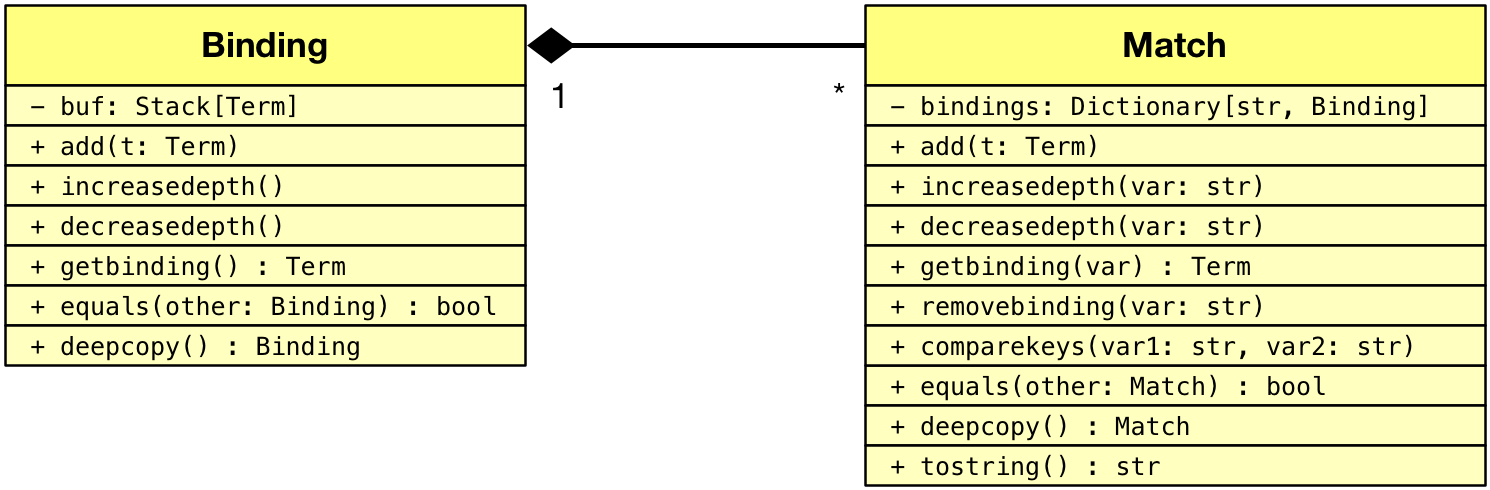
\includegraphics[scale=0.27]{class-diagram-match-binding.png} }
	\caption{\texttt{Match} and \texttt{Binding} class diagram.}
\label{class-diagram-match-binding}
\end{figure}

The \texttt{Binding} class encapsulates a stack of terms and provides three methods for its manipulation:

\begin{itemize}
\item 
\texttt{increase\_depth} pushes the term \texttt{Sequence} onto the stack provided a term on top of the stack is also a \texttt{Sequence}, otherwise it raises an Exception.

\item
\texttt{decrease\_depth} has the following behaviour:
	\begin{enumerate}
		\item
        if the stack is empty, raises an Exception.
		\item
		if the stack size is 1 and the topmost element is not a \texttt{Sequence}, raises an Exception.
		\item
		if the stack size is 1 and the topmost element is a \texttt{Sequence}, does nothing.
		\item
        if the stack size is greater than one, pops the topmost \texttt{Sequence} and append it to \texttt{Sequence} below. (this works because \texttt{increasedepth} must be called beforehand)
	\end{enumerate}

\item
\texttt{add(term)} has the following behaviour:
	\begin{enumerate}
		\item
         if the stack is empty, adds \texttt{term}. 
		\item
         if the stack is not empty and the topmost term is not \texttt{Sequence}, raises an Exception
		\item
        if the stack is not empty and the topmost term is \texttt{Sequence}, adds \texttt{term} to the \texttt{Sequence}.
	\end{enumerate}
\end{itemize}

\texttt{Match} class associates pattern-variable with \texttt{Binding} instance.

\begin{itemize}
\item
\texttt{increase\_depth} calls \texttt{increase\_depth} method of relevant \texttt{Binding} instance.

\item
\texttt{decrease\_depth} calls \texttt{decrease\_depth} method of relevant \texttt{Binding} instance.

\item
\texttt{addtobinding} calls \texttt{add} method of relevant \texttt{Binding} instance with \texttt{term}.

\item
\texttt{comparekeys(key1, key2)}. Given two keys, appropriate \texttt{Binding} instances are retrieved and then the topmost terms on the stack are compared.

\item
\texttt{deepcopy} creates a new \texttt{Match} with deep-copies of \texttt{Binding} and \texttt{Term}. 
\end{itemize}

\section{Processing Input}


\subsection{Lexical Analysis and Parsing}

Initially, input to PyPltRedex is read from the file and stored as a string. To be able to apply reduction-relation, the string needs to be analyzed. 

Lexical analysis breaks up the string into individual tokens and decides which kind of token it is. Most commonly tokens are described using regular expressions. 

Parsing takes individual lexemes and creates structured data out of them. In this case, \texttt{Term} instances are produced. 

The grammar can be seen in Figure \ref{tok-lex-grammar}.


\begin{figure}[h]
\begin{minted}[tabsize=2,obeytabs,escapeinside=::,mathescape=true,fontsize=\normalsize]{text}
term = term-sequence 
     | term-atom

term-sequence = lparen term* rparen

atom = (\#true|\#false|\#t|\#f)					  :$\langle boolean \rangle$:
	   | \"([^\"\\]|(\\[\s\S]))*\"				   :$\langle string  \rangle$:
	   | (\+|\-)?[0-9]*\.[0-9]+					    :$\langle float \rangle$:
	   | (\+|\-)?[0-9]+							        :$\langle integer \rangle$:
	   | ([^ \(\)\[\]\{\}\"\'`;\#\n])*
	     ([^ \(\)\[\]\{\}\"\'`;\#0123456789\n])+ 
	     ([^ \(\)\[\]\{\}\"\'`;\#\n])*       :$\langle identifier \rangle$:

lparen = [\[\{\(]             :$\langle opening \text{ } parentheses \rangle$:
rparen = [\]\}\)]             :$\langle closing \text{ } parentheses \rangle$:
\end{minted} 
\caption{Grammar for terms. All atoms match given regular expressions.}
\label{tok-lex-grammar}
\end{figure}

\subsection{Implementation}
Class diagram for both \texttt{Tokenizer} and \texttt{Parser} can be seen in Figure \ref{class-diagram-lexer-parser}.

\begin{figure}[h]
	\centering
	\makebox[\textwidth][c] { 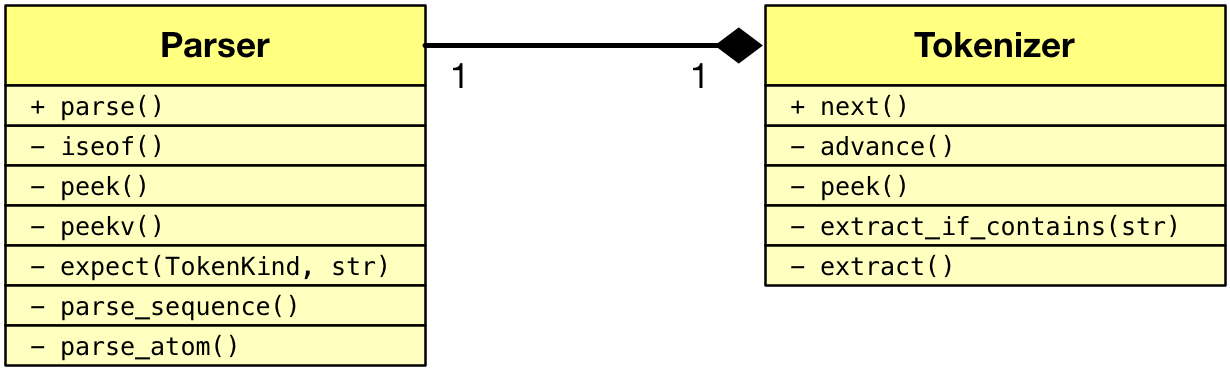
\includegraphics[scale=0.30]{class-diagram-lexer-parser.png} }
\caption{Class diagram for \texttt{Tokenizer} and \texttt{Parser}.}
\label{class-diagram-lexer-parser}
\end{figure}

Actual lexer implementation doesn't use regular expressions that were described above but implements their functionality using manually implemented state machine. Functions that classify characters can be seen in Figure \ref{char-predicates}.

\begin{figure}[h]
\begin{minted}[tabsize=2,obeytabs,escapeinside=::,mathescape=true,fontsize=\normalsize]{python}
def is_whitespace(c):
    return c == ' ' or c == '\t' or c == '\n' or c == '\r'

def is_newline(c):
    return c == '\n'

def is_reserved(c): 
    return c in ['(', ')', '[', ']', '{', '}', '\"', '\'', '`', ';', '#', '|', '\\']

def is_digit(c):
    return c in ['0', '1', '2', '3', '4', '5', '6', '7', '8', '9']

def is_plusminus(c):
    return c in ['-', '+']

def is_delimeteter(c):
    return is_reserved(c) or c == '\0' or is_whitespace(c)

def is_leftparen(c):
	return c in ['(', '[', '{']

def is_rightparen(c):
	return c in [')', ']', '}']
\end{minted}
\caption{Predicates for character identification.}
\label{char-predicates}
\end{figure}


\begin{itemize}
\item
\texttt{string} is the string that requires lexical analysis.

\item
\texttt{start} and \texttt{end} are indices indicating an interval within the \texttt{string}. The substring that ends with index \texttt{start} has already been analyzed. A substring between \texttt{start} and \texttt{end} is a potential token. Any substring after \texttt{end} requires analysis.

\item
\texttt{advance()} method increments \texttt{end} by one.

\item
\texttt{peek()} returns a character at index \texttt{end} of the \texttt{string}.

\item
\texttt{extract\_if\_contains(substring)} extracts substring \texttt{s} beginning at \texttt{start} and ending at \texttt{start+len(substring)} and compares it against provided \texttt{substring}. If both strings are equal, \texttt{start} and \texttt{end} indices are set to \texttt{start+len(substring)} and True is returned. Otherwise, False is returned.

\item
\texttt{extract()} extracts the string between \texttt{start} and \texttt{end}, sets \texttt{start=end} and returns the extracted string.

\item
	\texttt{next()} returns the next token in the string. This method implements actual tokenization logic. All regular expressions are implemented directly instead of using RPython's regular expression library (for reasons why see below). State machine representing this method can be seen in Figure \ref{lexical-analysis-tokenize}.

\begin{figure}[th!]
	\centering
	\makebox[\textwidth][c] { 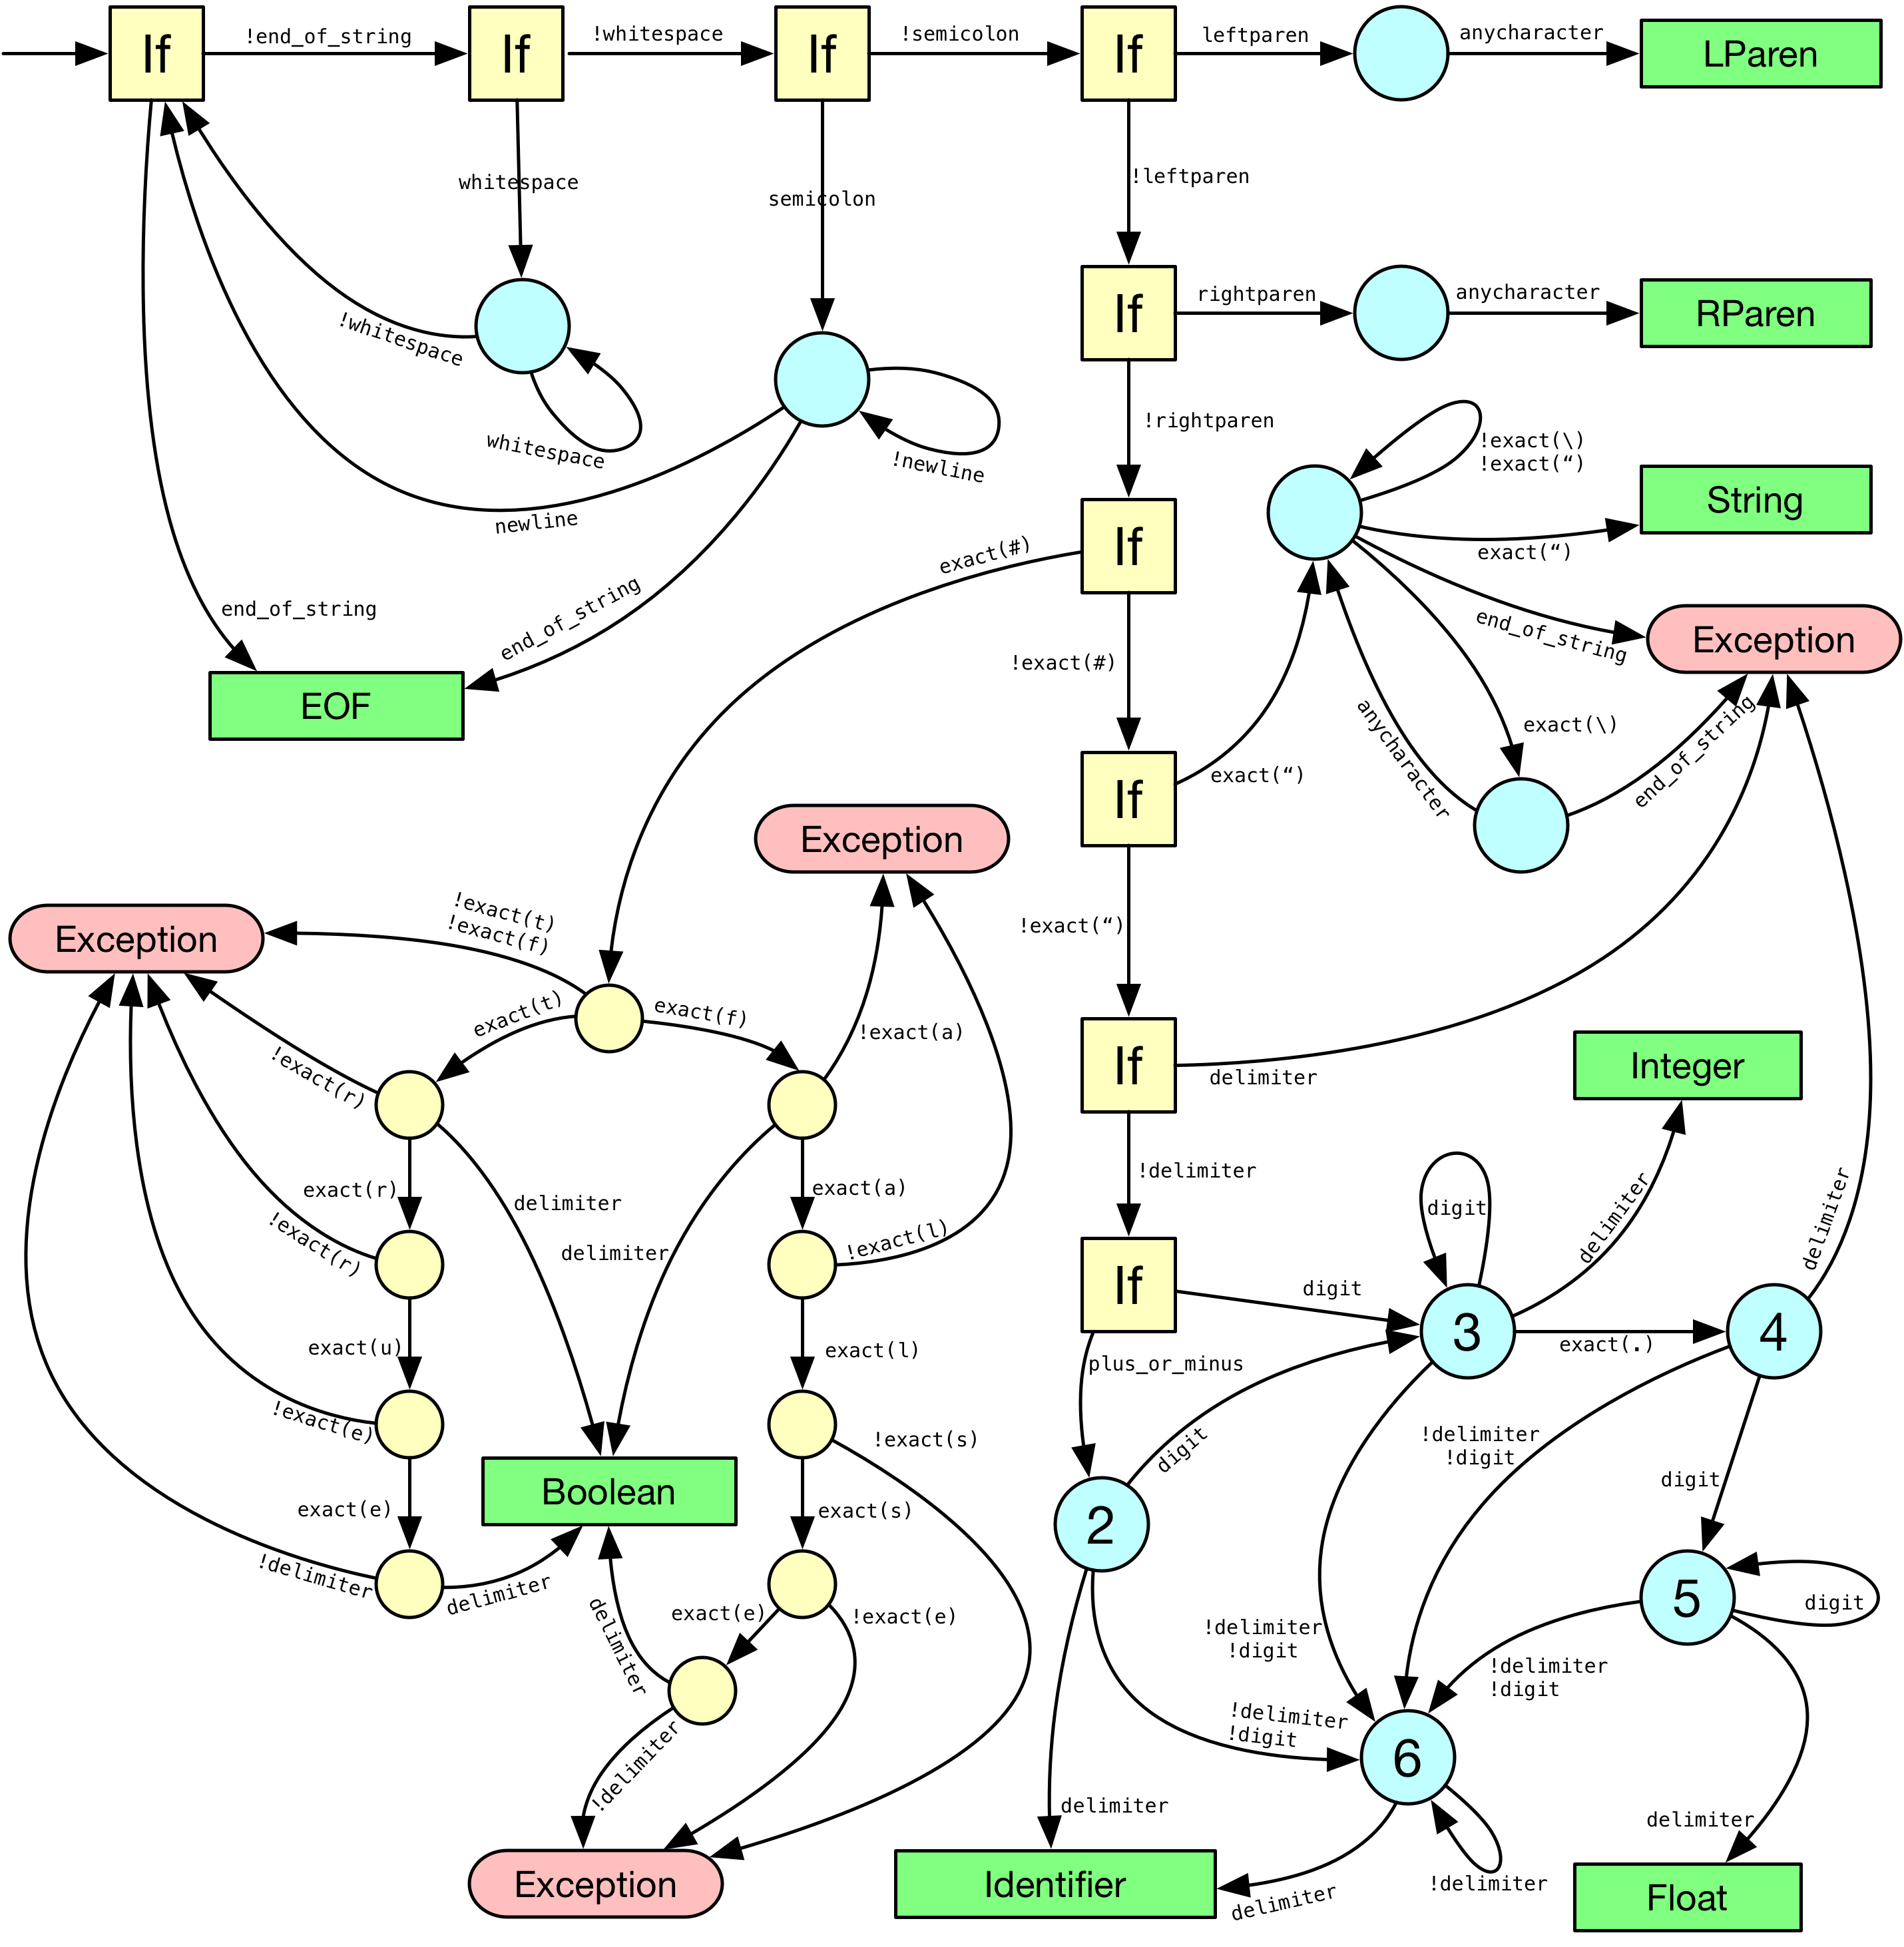
\includegraphics[scale=0.16]{lexical-analysis-tokenize.png} }
\caption{State machine for lexical analysis.}
\label{lexical-analysis-tokenize}
\end{figure}

Edges of the graph represent calls to \texttt{peek()} and ensuring the character satisfies a predicate an edge is labeled with. Taking a transition does not consume any characters. Predicates are described above.

The state machine has different node types with different character consumption strategies.
\begin{itemize}
\item states that return tokens annotated with their types, highlighted in green. After moving to this state no input is consumed.
\item states that raise Exceptions highlighted in red. After moving to this state no input is consumed.
\item \texttt{If} states are essentially \texttt{if} statements. They consume no characters.
\item Circled blue states actually consume characters. They also may have self-loops indicating consumption of one or more characters satisfying given predicate.
\item Circled yellow states are conceptually identical to blue states but are handled differently as explained below.
\end{itemize}

The state machine proceeds in the following manner

\begin{enumerate}
\item First ensure end of the string has not been reached, otherwise return (Eof)
\item Then, if current character whitespace, go to the state $s1$ that consumed all whitespace characters. Go back to the beginning and perform "end of the string" check.
\item After moving to state $if3$ and if current character is semicolon indicating beginning of comment, go to state $s2$ that consumes anything that is not a newline or end-of-the-string. Comment is then discarded and state machine transitions either to $if1$ or $eof$ returning (Eof).
\item Next two If statements detect closing and opening parantheses/braces/brackets and return (Lbrace) or (Rprace) accordingly.
\item If current character starts with pound sign indicating possible boolean, goto state $s3$. These yellow states do not consume input character by character but utilize \texttt{extract\_if\_contains} peek and consume multiple characters at once. This method is called in following manner:
\begin{itemize}
\item
if \texttt{extract\_if\_contains("\#t")} return (Boolean "\#t)
\item
if \texttt{extract\_if\_contains("\#f")} return (Boolean "\#f)
\item
if \texttt{extract\_if\_contains("\#true")} return (Boolean "\#t)
\item
if \texttt{extract\_if\_contains("\#false")} return (Boolean "\#f)
\end{itemize}

\item If current character is double quote, consume any character until closing double quote is found. Escape sequences are supported expecting a single character after backward slash. If end-of-string is encountered prematurely, Exception is raised. Otherwise, (String, \texttt{self.extract()}) is returned.

\item Finally, at this point a token can only be an integer, float, or identifier. This state machine is more complex.

\begin{itemize}
\item After arriving into state $1$, next character can either be (1) plus or minus thus moving to state 2;  (2) digit thus moving to state 3; (3) any other symbol that is not a delimeter this moving to state 6; and (4) delimiter thus moving to Exception state.
\item After arriving to state $2$ and consuming \texttt{+} or \texttt{-}, next character can either be (1) digit -> 3; (2) delimeter -> returning (Identifier, \texttt{extract()}) as \texttt{-} or \texttt{+} are valid identifiers in Racket; (3) Any other symbol that is not delimeter -> 6.
\item After arriving to state 3 and consuming a digit, next character can either be (1) a digit -> 3 (implemented as \texttt{while} loop); (2) delimeter thus returning (Integer, extract()); (3) fullstop symbol -> 4 indicating potential floating point number; (4) character that is neither a delimeter/number/nor fullstop -> 6.
\item After arriving to state 4 and consuming fullstop, next character can either be (1) delimeter -> raise Exception because fractional part of the float is missing; (2) digit -> 5; (3)neither a digit or delimeter -> 6.
\item After arriving to state 5 and consuming a digit, next character can either be (1) digit -> 5 (again, implemented as \texttt{while} loop); (2) delimeter -> return (Float, extract()) (3) neither a digit nor delimeter -> 6.
\item After arriving to state 6 and consuming some character, next character can either be (1) delimeter - return (Ident, extract()); (2) not delimeter -> 6.

\end{itemize}
This completes state machine description
\end{enumerate}

\end{itemize}

This completes description of the tokenizer. The parser is implemented as a very simple recursive descent parser. Below follows the description of its methods and their functionalities.

\begin{itemize}
\item
\texttt{iseof()} returns true if end of the string has been reached.

\item
\texttt{peek()} returns kind of the next token. 

\item
\texttt{peekv()} returns kind of the next token along with it's value.

\item 
\texttt{expect(expectedkind, tok=None)} throws Exception when \texttt{currenttoken} is not the one expected. In particular,
	\begin{itemize}
		\item
		If \texttt{expectedkind != nexttoken.kind} raise Exception.
		\item
		If \texttt{tok != None}, additionally check if \texttt{tok=nexttoken.value}. Raise Exception if it is not.
		\item
		Otherwise, call \texttt{tokenizer.next()} and assign it to \texttt{nexttoken} and return previous token. 
	\end{itemize}

\item 
	\texttt{parse\_sequence} implements parsing of \texttt{term-sequence} from the grammar above
	\begin{itemize}
		\item
		Let \texttt{seq} be an empty list.

		\item
		The first token is expected to be \texttt{LParen}.

		\item
		While \texttt{peek()} is not \texttt{RParen}, if \texttt{peek()} is \texttt{LParen}, call \texttt{term-sequence} and append its result to \texttt{seq}, otherwise call \texttt{parse\_atom} and append its result to seq.
	
		\item
		\texttt{expect(RParen)} 

		\item
		Return \texttt{Sequence(seq)}
	\end{itemize}

\item
\texttt{parse\_atom} implements parsing of \texttt{atom} from grammar.
	\begin{itemize}
	\item
		If \texttt{peek()} is Integer, return \texttt{Integer(expect(Integer))}
	\item
		If \texttt{peek()} is Float, return \texttt{Float(expect(Decimal))}
	\item

		If \texttt{peek()} is String, return \texttt{String(expect(String))}
	\item
		If \texttt{peek()} is Boolean, return \texttt{Boolean(expect(Boolean))}
	\item

		If \texttt{peek()} is Ident, then \texttt{peekv} to retrieve the value of the token. If value of token is \texttt{hole} return \texttt{Hole()}, otherwise Variable(self.expect(Ident)).
	\end{itemize}
	

\end{itemize}

\subsection{Implementation: Difficulties}
Initial lexical analysis implementation relied on regular expression library provided by RPython for identifying integers, floating point numbers and identifiers using regular expressions described in section TODO. While library works fine while running the lexer using \texttt{python2.7}, attempting to compile lexer code using \texttt{rpython} toolchain results in the following compilation error:

\begin{lstlisting}
[translation:ERROR] AttributeError: 'FrozenDesc' object has no attribute 'pycall'
Processing block:
 block@1149[_choice5_0...] is a <class 'rpython.flowspace.flowcontext.SpamBlock'> 
 in (rpython.rlib.parsing.regexparse:1495)RegexParser._charclass 
 containing the following operations: 
       v1 = simple_call((type set), v0) 
       v2 = simple_call((builtin_function range), (97), (123)) 
       v3 = newlist() 
       v4 = iter(v2) 
       v5 = hint(v3, v2, ({'maxlength': True})) 
\end{lstlisting}

Seems like RPython's \texttt{RegexParser} functionality has a bug. After attempting to investigate, I decided (TODO passive voice) to implement these regular expressions manually instead of relying on the library. This decision was made also because construction of those regular expressions was rather slow.

\subsection{Future Improvements}

Since lexical analysis and parsing were implemented very early on, some of the regular expressions were hacked together to make everything work in short amount of time. In certain cases tokenization is not performed correctly with respect to Racket's tokenization logic. For example, Racket allows for specification of floating point numbers such as \texttt{.045} or \texttt{1.} (that is there must be either a digit before or after a decimal), which current implementation doesn't support (and are identified as Identifier instead). Scientific notation isn't supported, either.

\section{Fresh Variable Generation}
PltRedex provides a very convinient form \texttt{(variables-not-in t p)}. Term \texttt{p} is expected to contain a single variable \texttt{v} such as \texttt{(term a)}. Given term \texttt{t}, \texttt{variables-not-in} form produces a term containing a fresh variable \texttt{v\_out} with prefix \texttt{p\_out} and some suffix \texttt{s\_out} such that there's no variable \texttt{v\_prime} in \texttt{t} with \texttt{v\_out = v\_prime}; or \texttt{v\_out not in Variables(t)} where \texttt{Variables(t)} is the set of all variables in \texttt{t}. Suffix \texttt{s\_out} may contain only digits or be empty. 

For example, variable \texttt{abc1xyz123} is decomposed into prefix \texttt{abc1xyz} and suffix \texttt{123}.

\subsection{Algorithm}
\begin{itemize}
\item
Initialize an empty dictionary.

\item
For each \texttt{v\_prime in Variables(t)}, try to decompose \texttt{v\_prime} into \texttt{p\_prime} and \texttt{s\_prime} interpreted as a number. 

	\begin{itemize}
	\item
	If such decomposition is possible, insert \texttt{(p\_prime, s\_prime)} into the dictionary. If \texttt{p\_prime} is not in the dictionary, initialize it to be an empty list and append \texttt{s\_prime} to it.

	\item
		Otherwise, insert \texttt{(v\_prime, -1)} into the dictionary \texttt{d}. If \texttt{v\_prime} is not in the dictionary, initialize it to be an empty list and append string -1 to it. Special value of -1 is used to indicate that \texttt{v\_prime} does not have a suffix.
	\end{itemize}

\item
Decompose \texttt{v} into prefix \texttt{p} and suffix \texttt{s}.

	\begin{itemize}
	\item
	If decomposition is not possible, check if \texttt{v} is in dictionary \texttt{d} and if it isn't return \texttt{Variable(v)}, meaning term \texttt{v} is not in \texttt{Variables(t)}.
	\item
	If decomposition is possible, check if \texttt{p} is in dictionary \texttt{d} and if it isn't return \texttt{Variable(v+s)}. Additionally, check if suffix \texttt{s} is in \texttt{d[p]}. If it isn't, return \texttt{Variable(v+s)}. This is done to return \texttt{a00} given \texttt{Variables(t) = \{a, a0\}} and \texttt{v=a00}, for example. Otherwise, let \texttt{v=p}.
	\end{itemize}

\item
Otherwise, the algorithm searches for a unique suffix by interpreting each suffix in \texttt{d[v]} as a number. Let \texttt{N} be list containing prefixes interpreted as a number and sorted in ascending order.  The goal is to find the smallest number \texttt{i > 0} that is not in \texttt{N}. If first \texttt{N[0]} is not \texttt{-1}, then \texttt{v} is not in \texttt{Variables(t)} and is already fresh. Return \texttt{Variable(v)}.

\item
Initialize \texttt{i=1} and \texttt{j=1}. \texttt{N[0]} is -1. Let \texttt{n} be the length of the list \texttt{N}. While \texttt{j<n}:
	\begin{itemize}
		\item
		If \texttt{i < N[j]} return \texttt{Variable(v+i)}.
		\item
		If \texttt{i > N[j]} then increment \texttt{j} by one. This case only happens when 0 is in \texttt{N}.
		\item
		If \texttt{i = N[j]} then increment both \texttt{i} and \texttt{j} by 1.
	\end{itemize}
\item
The end of the list is reached and \texttt{Variable(v+i)} is returned.
\end{itemize}






\chapter{Pattern Matching}

\chapter{Term Generation}

\chapter{Top-Level Forms}

TODO

\chapter{Testing and Evaluation}
TODO

\chapter{Conclusion} 

\section{Future Work}
\subsection{Ellipsis Determinism}
In Chapter < Pattern codegen > an algorithm for deterministic matching of patterns under ellipsis was described but careful reader might notice the report doesn't describe how such patterns are made deterministic. In fact, PyPltRedex provides a transformation pass called \texttt{EllipsisMatchModeRewriter} that analyzes patterns under ellipses and decides if given ellipsis can be matched deterministically but current algorithm is flawed and doesn't work correctly for all patterns. 


\subsection{\texttt{define-metafunction} and \texttt{define-reduction-relation} pattern merging.}

Algorithms for application of reduction-relation and metafunctions match each pattern separately. However, it may be the case that patterns in reduction-cases are similar and bind terms to same identifiers in the same position within the pattern.

\begin{lstlisting}
(M_1  (in-hole P x (+ n_1 n_2)))
(M_1  (in-hole P n (- n_1 n_2)))
\end{lstlisting}

Two patterns above are an example - both patterns contain pattern-variable $M\_1$ in the first position within the sequence. This means at this point there needs to be a single $Match$ object containing $M\_1$. Since $in-hole$ patterns are different, after matching $M\_1$ $Match$ object can be copied to contain terms matches by each $in-hole$. Diagram can be seen below - 

TODO


Furthermore, the first pattern in both \texttt{in-hole} patterns is the same - $P$. Since both \texttt{in-hole} patterns are at the second position within respective pattern sequences, instead of using multiple term traversals to find child terms matching \texttt{(+ n\_1 n\_2)} and \texttt{(- n\_1 n\_2)}, one travesal would be sufficient. This could be done by introducing a new pattern, say, $InHoleMulti(pattern1, pattern2 ...)$ that accepts multiple patterns. Diagram for this can be seen below:

TODO


However, since since matches may have been split before, this introduces additional complexity of \texttt{Match} object management.

\subsection{More evaluation}

I was not able to explore performance of the system w.r.t. larger terms.





\chapter{ListListing example}
\lstset{language=algebra,linewidth=0.95\linewidth,breaklines=true,numbers=left,
basicstyle=\ttfamily,numberstyle=\tiny,escapeinside={//*}{\^^M},
mathescape=true}
\begin{lstlisting}
import IntSpec, ItemSpec;

sort cart; //*\label{sort}

constructors //*\label{begin-sig}
create() $\longrightarrow$ cart;
insert(cart, item) $\longrightarrow$ cart;
observers
amount(cart) $\longrightarrow$ int;
transformers
delete(cart, item) $\longrightarrow$ cart; //*\label{end-sig}

axioms //*\label{begin-axioms}
forall c: cart, i, j: item 

amount(create()) $=$ 0; //*\label{begin-amount}
amount(insert(c,i)) $=$ amount(c) $+$ price(i); //*\label{end-amount}
delete(create(),i) $=$ create(); //*\label{begin-delete}
delete(insert(c,i),j) $=$
if (i =$\:$= j) c
else insert(delete(c,j),i); //*\label{end-axioms}
end
\end{lstlisting}



\backmatter

\chapter{Glossary} %optional

%\bibliographystyle{alpha}
%\bibliographystyle{dcu}
\bibliographystyle{plainnat}
\bibliography{biblio}

%\cleardoublepage
%\theindex %optional, use only if you have an index, must use
	  %\makeindex in the preamble
\lipsum

\end{document}
